%
%	Задача Коши для систем дифференциальных уравнений
%
\newpage
\section{Задача Коши для систем 
обыкновенных дифференциальных уравнений}
При рассмотрении физических явлений и процессов часто 
не удается найти непосредственную взаимосвязь между 
величинами, характеризующими эволюционный, 
т.е. изменяющийся во времени, процесс. 
Однако во многих случаях можно установить связь между 
искомыми характеристиками изучаемого явления (функциями) 
и скоростями их изменения относительно других переменных, 
т.е. найти уравнения, в которые входят производные от
неизвестных функций. Такие уравнения называют 
\emph{дифференциальными}. 

Задача Коши обычно возникает при анализе процессов, 
определяемых дифференциальным законом эволюции и 
начальным состоянием (начальным условием) 
и для системы обыкновенных дифференциальных уравнений 
эта задача формулируется в виде системы уравнений:
\begin{gather}\label{eq:ODE_SYS}
\diff{\vect{u}}{t} = \vect{f}(t, \vect{u}),
\quad
\vect{u}(0)=\mathring{\vect{u}},
\end{gather}
где $\vect{u}(t)$ -- неизвестные функции, которые подлежат 
определению;
$\vect{f}(t, \vect{u})$ -- известные функции, 
зависящие от времени и неизвестных функций;
$\mathring{\vect{u}}$ -- \emph{начальные условия}, 
т.е. значения неизвестных функций в начальный момент времени 
$(t=0)$. 

Система обыкновенных дифференциальных 
уравнений первого порядка и начальные условия
\eqref{eq:ODE_SYS} в развернутом виде могут быть 
записаны как:
\begin{gather}\label{eq:ODE_IC}
\left\{\begin{matrix}
\diff{u_1}{t}&=&f_1(t, u_1,u_2,\cdots,u_n),&u_1(0)&=&\mathring u_1\\[1em]
\diff{u_2}{t}&=&f_2(t, u_1,u_2,\cdots,u_n),&u_2(0)&=&\mathring u_2\\[1em]
\hdotsfor{1}&=&\hdotsfor{1}&\hdotsfor{1}&=&\dots\\[1em]
\diff{u_n}{t}&=&f_n(t, u_1,u_2,\cdots,u_n),&u_n(0)&=&\mathring u_n
\end{matrix}\right.,
\end{gather}
где $n$ -- количество дифференциальных уравнений 
в системе \eqref{eq:ODE_SYS}.

Точное решение систем дифференциальных уравнений 
вида \eqref{eq:ODE_IC}, которые описывают 
многообразие прикладных задач, может быть 
получено лишь в исключительных случаях. 
Поэтому возникает необходимость 
\emph{приближенного решения} таких задач. 
В настоящее время создано и разработано 
значительное число приближенных методов решения 
дифференциальных уравнений, каждый из которых имеет 
свои преимущества и недостатки.

%
% Метод Эйлера
%
\emptyline
\subsection{Метод Эйлера решения задачи Коши}
Будем полагать, что решение задачи Коши \eqref{eq:ODE_IC} существует, 
единственно и обладает необходимыми свойствами гладкости.

Введем временную сетку, т.е. будем
рассматривать изменения неизвестных функций 
только в заданные моменты времени:
\begin{gather*}
\{t_j\},\quad j=1,2,\dots N,
\end{gather*}
где $j$ -- номер временного интервала;
$\Delta t_{j+1} = (t_{j+1}-t_j)$ -- шаг сетки, т.е. временной интервал 
между двумя последовательными моментами времени;
$N$ -- количество узлов временной сетки.

Основная идея метода Эйлера заключается в предположении, 
о том что неизвестные функции $\vect{u}(t)$ изменяются линейно
в интервале $[t_j,t_{j+1}]$ между двумя соседними узлами 
временной сетки и интерполяция неизвестных функций 
проводится полиномом первого порядка $\vect{L}_1(t)$:
\begin{gather*}
\vect{u}(t)\approx\vect{L}_1(t)=
\dfrac{t-t_{j+1}}{t_j-t_{j+1}}\cdot\vect{u}(t_j)+
\dfrac{t-t_j}{t_{j+1}-t_j}\cdot\vect{u}(t_{j+1}).
\end{gather*}

Производная от неизвестной функции приближенно 
аппроксимируется выражением вида:
\begin{gather}
\diff{\vect{u}}{t}\approx\vect{L}^{\prime}_1(t) =
\dfrac{\vect{u}(t_{j+1})-\vect{u}(t_j)}{t_{j+1}-t_j},
\end{gather}
где $t_{j+1}$ и $t_j$ -- два последовательных момента времени.

Тогда систему дифференциальных уравнений первого порядка 
\eqref{eq:ODE_SYS} приближенно можно записать в виде:
\begin{gather}\label{eq:ODE_NUM}
\dfrac{\vec u(t_{j+1})-\vec u(t_{j})}{\Delta t_{j+1}}\approx
\vec f\left(t_j, \vec u(t_{j})\right)
\end{gather}

Относительно неизвестных $\vec u(t_{j+1})$ 
это система линейных алгебраических уравнений и 
решение системы \eqref{eq:ODE_NUM} находится явным образом 
по рекуррентным формулам:
\begin{gather}\label{eq:ODE_EULER}
\vec u(t_{j+1})=\vec u(t_{j})+\Delta t_{j+1}\cdot\vec f\left(t_j, \vec u(t_{j})\right),
\quad \vec{u}(0)=\vec{\mathring u}.
\end{gather}

Метод Эйлера является простейшим численным методом 
решения задачи Коши. К недостаткам метода можно отнести
малую точность и систематическое накопление ошибок.

Для простоты рассмотрим только одно дифференциальное уравнение 
с единственным начальным условием:
\begin{gather*}
y(t_{j+1})=y(t_{j})+\Delta t_{j+1}\cdot f\left(t_j, y(t_{j})\right),
\quad y(0)=\mathring y
\end{gather*}

На рисунке \ref{fig:EULER} представлена графическая иллюстрация 
метода Эйлера численного решения задачи Коши 
для одного дифференциального уравнения первого порядка.
% *******************************
%	Ломаная Эйлера
%
\begin{figure}[H]\centering
\begin{tikzpicture}
\begin{axis}[% оси координат
xlabel=\empty,ylabel=\empty,
xmin=-1,xmax=11,xtick={0,2,4,6,8,10},xticklabels={$0$,$t_1$,,$t_j$,,$t_N$},
ymin=0.5,ymax=7,ytick={1,2.5,3.5,5,6,6.5},yticklabels={$\mathring{y}$,$y(t_1)$,,$y(t_j)$,,$y(t_N)$},
width=10cm,
name=GRAPH]
\addplot[ball darkblue] coordinates 
{(0,1) (2,2.5) (3,3.5) (6,5) (8,6) (10,6.5)}
node[pos=0.2,color=darkblue,below right] 
{$y(t_1)=\mathring{y}+\Delta t_1\cdot f(0,\mathring{y})$}
node[pos=0.3,color=darkblue,below right] 
{$y(t_2)=y(t_1)+\Delta t_2\cdot f(t_1,y(t_1))$};
\end{axis}
%\draw[thick,red] ($(GRAPH.south)-(0,2em)$) node {a};
\end{tikzpicture}\\
a)
%\par пример
\caption{Ломаная Эйлера}
\label{fig:EULER}
\end{figure}
% *******************************

%
%	Оценка погрешности решения задачи Коши
%
\subsection{Оценка погрешности решения задачи Коши}
Интегрирование системы дифференциальных уравнений 
\eqref{eq:ODE_SYS} по временной переменной $t$ 
с учетом начальных условий:
\begin{gather}\label{eq:ODE_SYS_INT}
\vec{v}(t)=\vec{u}(0)+\int\limits_{0}^{t}\vec f(\xi, \vec{v})d\xi.
\end{gather}

Уравнение \eqref{eq:ODE_SYS_INT} является 
интегральным уравнением для неизвестной функции $\vec{v}(t)$,
а его решение эквивалентно решению задачи Коши 
\eqref{eq:ODE_SYS}, что можно проверить прямой подстановкой
\eqref{eq:ODE_SYS_INT} в \eqref{eq:ODE_SYS}.

На временной сетке $\{t_j\}$ интеграл в правой части равенства 
\eqref{eq:ODE_SYS_INT} приближенно вычисляется по 
\emph{формуле трапеций}:
\begin{gather}\label{eq:ODE_SYS_INT_TRAP}
\int\limits_{0}^{t_{j+1}}\vec f(\xi, \vec{v})d\xi\approx
\sum\limits_{k=0}^{j}
\dfrac{
\vec f\left(t_{k+1},\vec{v}(t_{k+1})\right)+
\vec f\left(t_{k},\vec{v}(t_{k})\right)
}{2}\cdot(t_{k+1}-t_k).
\end{gather}

Воспользовавшись \eqref{eq:ODE_SYS_INT_TRAP}, 
выражение для решения интегрального уравнения 
\eqref{eq:ODE_SYS_INT} можно записать 
в рекуррентной форме:
\begin{gather}\label{eq:ODE_INT_EQ}
\vec{v}(t_{j+1})=\vec{v}(t_{j})+
\dfrac{
\vec f\left(t_{j+1},\vec{v}(t_{j+1})\right)+
\vec f\left(t_{j},\vec{v}(t_{j})\right)
}{2}\cdot\Delta t_{j+1}.
\end{gather}

Для определения приближенного значения решения 
интегрального уравнения \eqref{eq:ODE_INT_EQ}
могут быть использованы значения неизвестных функций 
${\vec u}(t_{j})$, рассчитанные по методу Эйлера
\eqref{eq:ODE_EULER} на $j$-ом временном слое:
\begin{gather}
\vec{v}(t_{j+1})\approx\vec{v}(t_{j})+
\dfrac{
\vec f\left(t_{j+1},{\vec u}(t_{j+1})\right)+
\vec f\left(t_{j},{\vec u}(t_{j})\right)
}{2}\cdot\Delta t_{j+1}.
\end{gather}

В качестве предельной абсолютной погрешности 
приближенного решения ${\vec u}(t_{j})$ 
задачи Коши \eqref{eq:ODE_SYS} можно принять величину:
\begin{gather}
\varepsilon_i(t_j)=|v_i(t_j) - {u}_i(t_j)|,\quad i=1,2,\dots n
\end{gather}

Контроль точности приближенного решения 
может вестись покомпонентно или по норме.
Для различных компонент решения задачи $\vec{u}_i$ 
могут использоваться различные допустимые значения 
погрешности.

Контроль точности по норме означает, что контролируется 
некоторая определенная норма оценки погрешности:
\begin{gather*}
\norma{\varepsilon}_{\infty}=\max_{i=1..n} \varepsilon_i
\quad
\norma{\varepsilon}_1=\sum\limits_{i=1}^n \varepsilon_i,
\quad
\norma{\varepsilon}_2=\sqrt{\sum\limits_{i=1}^n \varepsilon_i^2}
\end{gather*}


%
%	Численное решение задачи Коши методом Эйлера
%
\subsection{Численное решение задачи Коши методом Эйлера}

Применяя метод Эйлера, найдем решение задачи Коши
системы дифференциальных уравнений:
\begin{gather}\label{eq:ODE_MY}
\left\{\begin{matrix}
\diff{u_1}{t}&=&{0,2}t+u_2,&u_1(0)&=&1\\[1em]
\diff{u_2}{t}&=&-\dfrac{u_1}{2},&u_2(0)&=&0
\end{matrix}\right.
,\end{gather}
в пределах отрезка $t\in[0, 10]$ на равномерной сетке с количеством временных интервалов $N=5$.

Введем обозначения
\begin{gather*}
\left\{\begin{array}{rcl}
f_1(t)&=&{0,2}\cdot{t}+u_2(t)\\[1em]
f_2(t)&=&-\dfrac{u_1(t)}{2}
\end{array}\right.
.\end{gather*}
где $f_1$ и $f_2$ -- функции, стоящие в правых частях 
дифференциальных уравнений системы \eqref{eq:ODE_MY}:

Рекуррентные соотношения \eqref{eq:ODE_EULER_SYS} 
для решения задачи Коши \eqref{eq:ODE_MY} методом Эйлера:
\begin{gather}\label{eq:ODE_SYS_RR}
\left\{\begin{matrix}
u_1(t_{j+1})&=&u_1(t_{j})+\tau\cdot f_1(t_j),&u_1(0)&=&1\\%[1em]
u_2(t_{j+1})&=&u_2(t_{j})+\tau\cdot f_2(t_j),&u_2(0)&=&0
\end{matrix}\right.
,\end{gather}

Решение системы интегральных уравнений \eqref{eq:ODE_SYS_INT} 
определяется рекурретными соотношениями:
\begin{gather}\label{eq:ODE_SYS_INT_RR}
\left\{\begin{matrix}
\hat{u}_1(t_{j+1})&=&\hat{u}_1(t_{j})+\tau\cdot\dfrac{f_1(t_{j})+f_1(t_{j+1})}{2},&\hat{u}_1(0)&=&1\\[1em]
\hat{u}_2(t_{j+1})&=&\hat{u}_2(t_{j})+\tau\cdot\dfrac{f_2(t_{j})+f_2(t_{j+1})}{2},&\hat{u}_2(0)&=&0
\end{matrix}\right.
.\end{gather}

Определим временной шаг метода Эйлера, зная длину временного отрезка (``время наблюдения``) 
и количество интервалов:
\begin{gather*}
\tau=\dfrac{t_{max}-t_0}{N} = \dfrac{10-0}{5}=2
,\end{gather*}
где $t_0=0$ -- начальный момент времени;
$t_{\max}$ -- максимальное время (``время наблюдения``).

Введем по переменной $t$ равномерную сетку с шагом $\tau=2$:
\begin{gather*}
\{t_j\}=\{0,2,4,6,8,10\}
\end{gather*}

Последовательно определяем приближенное решение 
задачи Коши \eqref{eq:ODE_MY} методом Эйлера,
используя рекуррентные соотношения \eqref{eq:ODE_SYS_RR}.
\begin{enumerate}
\item
Определим значения неизвестных функций $u_1$ и $u_2$ в точке $t_1=2$:
\begin{gather*}\begin{array}{rcl}
f_1(0)&=&{0,2}\cdot0+u_2(0)={0,2}\cdot0+0=0\\[1em]
f_2(0)&=&-\dfrac{u_1(0)}{2}=-\dfrac{1}{2}=-0,5
\end{array}\end{gather*}
%
\begin{gather*}
\left\{\begin{array}{rcl}
u_1(2)&=&u_1(0)+2\cdot{f_1(0)}=1+2\cdot0=1\\[1em]
u_2(2)&=&u_2(0)+2\cdot{f_2(0)}=0+2\cdot(-0,5)=-1
\end{array}\right.
.\end{gather*}
\item
Определим значения неизвестных функций $u_1$ и $u_2$ в точке $t_2=4$:
\begin{gather*}\begin{array}{rcl}
f_1(2)&=&{0,2}\cdot2+u_2(2)={0,2}\cdot2+(-1)=-0,6\\[1em]
f_2(2)&=&-\dfrac{u_1(2)}{2}=-\dfrac{1}{2}=-0,5
\end{array}\end{gather*}
%
\begin{gather*}
\left\{\begin{array}{rcl}
u_1(4)&=&u_1(2)+2\cdot{f_1(2)}=1+2\cdot(-0,6)=-0,2\\[1em]
u_2(4)&=&u_2(2)+2\cdot{f_2(2)}=-1+2\cdot(-0,5)=-2
\end{array}\right.
.\end{gather*}
\item
Определим значения неизвестных функций $u_1$ и $u_2$ в точке $t_3=6$:
\begin{gather*}
\begin{array}{rcl}
f_1(4)&=&{0,2}\cdot4+u_2(4)={0,2}\cdot4+(-2)=-1,2\\[1em]
f_2(4)&=&-\dfrac{u_1(4)}{2}=-\dfrac{-0,2}{2}=0,1
\end{array}\end{gather*}
%
\begin{gather*}
\left\{\begin{array}{rcl}
u_1(6)&=&u_1(4)+2\cdot{f_1(4)}=-0,2+2\cdot(-1,2)=-2,6\\[1em]
u_2(6)&=&u_2(4)+2\cdot{f_2(4)}=-2+2\cdot(0,1)=-1,8
\end{array}\right.
.\end{gather*}
\item
Определим значения неизвестных функций $u_1$ и $u_2$ в точке $t_4=8$:
\begin{gather*}\begin{array}{rcl}
f_1(6)&=&{0,2}\cdot6+u_2(6)={0,2}\cdot6+(-1,8)=-0,6\\[1em]
f_2(6)&=&-\dfrac{u_1(6)}{2}=-\dfrac{-2,6}{2}=1,3
\end{array}\end{gather*}
%
\begin{gather*}
\left\{\begin{array}{rcl}
u_1(8)&=&u_1(6)+2\cdot{f_1(4)}=-2,6+2\cdot(-0,6)=-3,8\\[1em]
u_2(8)&=&u_2(6)+2\cdot{f_2(6)}=-1,8+2\cdot(1,3)=0,8
\end{array}\right.
.\end{gather*}
\item
Определим значения неизвестных функций $u_1$ и $u_2$ в точке $t_5=10$:
\begin{gather*}\begin{array}{rcl}
f_1(8)&=&{0,2}\cdot8+u_2(8)={0,2}\cdot8+0,8=2,4\\[1em]
f_2(8)&=&-\dfrac{u_1(8)}{2}=-\dfrac{-3,8}{2}=1,9
\end{array}\end{gather*}
%
\begin{gather*}
\left\{\begin{array}{rcl}
u_1(10)&=&u_1(10)+2\cdot{f_1(4)}=-3,8+2\cdot(2,4)=1\\[1em]
u_2(10)&=&u_2(8)+2\cdot{f_2(8)}=0,8+2\cdot(1,9)=4,6
\end{array}\right.
.\end{gather*}
\end{enumerate}

На рисунке \ref{fig:u(t)} представлено решение задачи Коши 
системы дифференциальных уравнений \eqref{eq:ODE_MY}.
% *******************************
%	График функций
%
\begin{figure}
\begin{center}
\begin{tikzpicture}[background rectangle/.style={fill=olive!10}, show background rectangle]
\begin{axis}[
	every axis/.style={color=black, solid, thick},
	xlabel = {$t$},	% подпись оси x
	ylabel = {$u_1, u_2$},	% подпись оси y
	xmin=-0.5, xmax=11, xtick={0,2,4,6,8,10}, %xticklabels={$0$,$t_1$,,$t_j$,,$t_N$},
	ymin=-4, ymax=5, ytick={-4,-2,0,1,2,4,5}, %yticklabels={$y^{(0)}$,$y^{(1)}$,,$y^{(j)}$,,$y^{(N)}$},
	xtick style={thick, black},
	ytick style={thick, black},
	grid=major,		
	major grid style={color=black!20, dashed, thin},
	legend pos={north west},
]
\addplot[thick, mark=*, mark size=4pt, mark options={fill=yellow, draw=black, solid}] coordinates 
{(0,1) (2,1) (4,-0.2) (6,-2.6) (8,-3.8) (10,1)};
\addlegendentry{$u_1$};
\addplot[thick, mark=square*, mark size=3pt, mark options={fill=green, draw=black, solid}] coordinates 
{(0,0) (2,-1) (4,-2) (6,-1.8) (8,0.8) (10,4.6)};
\addlegendentry{$u_2$};
\end{axis}
\end{tikzpicture}
\end{center}
\caption{Зависимость неизвестных функций от времени}
\label{fig:u(t)}
\end{figure}
% *******************************

%
%	Приближенное решение интегрального уравнения
%
Последовательно определяем приближенное решение 
интегрального уравнения \eqref{eq:ODE_MY},
используя рекуррентные соотношения \eqref{eq:ODE_SYS_INT_RR}.
\begin{enumerate}[leftmargin = 1ex]
\item
Определим значения неизвестных функций $\hat{u}_1$ и $\hat{u}_2$ в точке $t_1=2$:
\begin{gather*}
\left\{\begin{array}{rcl}
\hat{u}_1(2)&=&\hat{u}_1(0)+\tau\cdot\dfrac{f_1(0)+f_1(2)}{2}
=1+2\cdot\dfrac{0+(-0,6)}{2}=0,4\\[1em]
\hat{u}_2(2)&=&\hat{u}_2(0)+\tau\cdot\dfrac{f_2(0)+f_2(2)}{2}
=0+2\cdot\dfrac{-0,5+(-0,5)}{2}=-1
\end{array}\right.
.\end{gather*}
\item
Определим значения неизвестных функций $\hat{u}_1$ и $\hat{u}_2$ в точке $t_2=4$:
\begin{gather*}
\left\{\begin{array}{rcl}
\hat{u}_1(4)&=&\hat{u}_1(2)+\tau\cdot\dfrac{f_1(2)+f_1(4)}{2}
=0,4+2\cdot\dfrac{(-0,6)+(-1,2)}{2}=-2,4\\[1em]
\hat{u}_2(4)&=&\hat{u}_2(2)+\tau\cdot\dfrac{f_2(2)+f_2(4)}{2}
=-1+2\cdot\dfrac{-0,5+0,1}{2}=-1,4
\end{array}\right.
.\end{gather*}
\item
Определим значения неизвестных функций $\hat{u}_1$ и $\hat{u}_2$ в точке $t_3=6$:
\begin{gather*}
\left\{\begin{array}{rcl}
\hat{u}_1(6)&=&\hat{u}_1(4)+\tau\cdot\dfrac{f_1(4)+f_1(6)}{2}
=-2,4+2\cdot\dfrac{-1,2+(-0,6)}{2}=-4,2\\[1em]
\hat{u}_2(6)&=&\hat{u}_2(4)+\tau\cdot\dfrac{f_2(4)+f_2(6)}{2}
=-1,4+2\cdot\dfrac{0,1+1,3}{2}=0
\end{array}\right.
.\end{gather*}
\item
Определим значения неизвестных функций $\hat{u}_1$ и $\hat{u}_2$ в точке $t_4=8$:
\begin{gather*}
\left\{\begin{array}{rcl}
\hat{u}_1(8)&=&\hat{u}_1(6)+\tau\cdot\dfrac{f_1(6)+f_1(8)}{2}
=-4,2+2\cdot\dfrac{-0,6+2,4}{2}=-2,4\\[1em]
\hat{u}_2(8)&=&\hat{u}_2(6)+\tau\cdot\dfrac{f_2(6)+f_2(8)}{2}
=0+2\cdot\dfrac{1,3+1,9}{2}=3,2
\end{array}\right.
.\end{gather*}
\item
Определим значения неизвестных функций $\hat{u}_1$ и $\hat{u}_2$ в точке $t_5=10$:
\begin{gather*}\begin{array}{rcl}
f_1(10)&=&{0,2}\cdot10+u_2(10)={0,2}\cdot8+4,6=6,2\\[1em]
f_2(10)&=&-\dfrac{u_1(10)}{2}=-\dfrac{1}{2}=-0,5
\end{array}\end{gather*}
%
\begin{gather*}
\left\{\begin{array}{rcl}
\hat{u}_1(10)&=&\hat{u}_1(8)+\tau\cdot\dfrac{f_1(8)+f_1(10)}{2}
=-2,4+2\cdot\dfrac{2,4+6,2}{2}=6,2\\[1em]
\hat{u}_2(10)&=&\hat{u}_2(8)+\tau\cdot\dfrac{f_2(8)+f_2(10)}{2}
=3,2+2\cdot\dfrac{1,9+(-0,5)}{2}=4,6
\end{array}\right.
.\end{gather*}
\end{enumerate}

На рисунке \ref{fig:uu(t)} представлены решения задачи Коши \eqref{eq:ODE_SYS} и
интегрального уравнения \eqref{eq:ODE_SYS_INT}, 
рассчитанные в различные моменты времени.

В таблице \ref{tab:error} и на рисунке \ref{fig:error} представлены значения
предельной абсолютной погрешности приближенного решения задачи Коши 
для различных моментов времени.
% *******************************
%	График функций
%
\begin{figure}[H]
\begin{center}
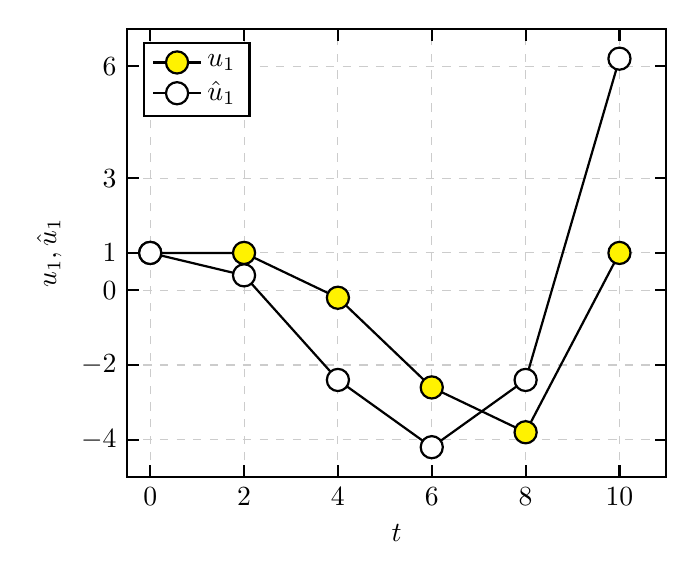
\begin{tikzpicture}
\begin{axis}[
	every axis/.style={color=black, solid, thick},
	xlabel = {$t$},	% подпись оси x
	ylabel = {$u_1, \hat{u}_1$},	% подпись оси y
	xmin=-0.5, xmax=11, xtick={0,2,4,6,8,10}, %xticklabels={$0$,$t_1$,,$t_j$,,$t_N$},
	ymin=-5, ymax=7, ytick={-4,-2,0,1,3,6}, %yticklabels={$y^{(0)}$,$y^{(1)}$,,$y^{(j)}$,,$y^{(N)}$},
	xtick style={thick, black},
	ytick style={thick, black},
	grid=major,		
	major grid style={color=black!20, dashed, thin},
	legend pos={north west},
]
\addplot[thick, mark=*, mark size=4pt, mark options={fill=yellow, draw=black, solid}] coordinates 
{(0,1) (2,1) (4,-0.2) (6,-2.6) (8,-3.8) (10,1)};
\addlegendentry{$u_1$};
\addplot[thick, mark=*, mark size=4pt, mark options={fill=white, draw=black, solid}] coordinates 
{(0,1) (2,0.4) (4,-2.4) (6,-4.2) (8,-2.4) (10,6.2)};
\addlegendentry{$\hat{u}_1$};
\end{axis}
\end{tikzpicture}
\end{center}
% *******************************
%	График функций
%
\begin{center}
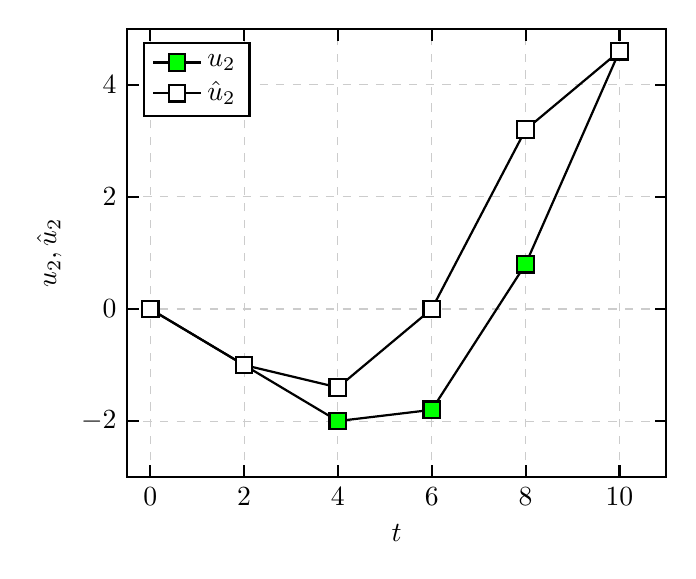
\begin{tikzpicture}
\begin{axis}[
	every axis/.style={color=black, solid, thick},
	xlabel = {$t$},	% подпись оси x
	ylabel = {$u_2, \hat{u}_2$},	% подпись оси y
	xmin=-0.5, xmax=11, xtick={0,2,4,6,8,10}, %xticklabels={$0$,$t_1$,,$t_j$,,$t_N$},
	ymin=-3, ymax=5, ytick={-2,0,2,4}, %yticklabels={$y^{(0)}$,$y^{(1)}$,,$y^{(j)}$,,$y^{(N)}$},
	xtick style={thick, black},
	ytick style={thick, black},
	grid=major,		
	major grid style={color=black!20, dashed, thin},
	legend pos={north west},
]
\addplot[thick, mark=square*, mark size=3pt, mark options={fill=green, draw=black, solid}] coordinates 
{(0,0) (2,-1) (4,-2) (6,-1.8) (8,0.8) (10,4.6)};
\addlegendentry{$u_2$};
\addplot[thick, mark=square*, mark size=3pt, mark options={fill=white, draw=black, solid}] coordinates 
{(0,0) (2,-1) (4,-1.4) (6,0) (8,3.2) (10,4.6)};
\addlegendentry{$\hat{u}_2$};
\end{axis}
\end{tikzpicture}
\end{center}
\caption{Приближенное решение задачи Коши и соответствующего интегрального уравнения}
\label{fig:uu(t)}
\end{figure}

\begin{table}
\caption{Предельная абсолютная погрешность приближенного решения задачи Коши \eqref{eq:ODE_MY}}
\label{tab:error}
\begin{tabular}{p{3cm} *{6}{p{1.5cm}}}
\toprule[1pt]
Время&0&2&4&6&8&10\\
\midrule
\multicolumn{7}{l}{Задача Коши}\\
\midrule
$u_1$&1&1&-0,2&-2,6&-3,8&1\\
$u_2$&0&-1&-2&-1,8&0,8&4,6\\
\midrule
\multicolumn{7}{l}{Интегральное уравнение}\\
\midrule
$\hat{u}_1$&1&0,4&-2,4&-4,2&-2,4&6,2\\
$\hat{u}_2$&0&-1&-1,4&0&3,2&4,6\\
\midrule
\multicolumn{7}{l}{Абсолютная погрешность $\epsilon=|\hat{u}-u|$}\\
\midrule
$\epsilon_1$&0&0,6&2,2&1,6&1,4&5,2\\
$\epsilon_2$&0&0&0,6&1,8&2,4&0\\
\bottomrule[1pt]
\end{tabular}
\end{table}

Из рисунка \ref{fig:error} видно, что максимальная 
предельная абсолютная погрешность для $u_1(t)$ 
составляет $\epsilon_1=5,1$, 
а для функции $u_2(t)$ -- $\epsilon_2=2,4$.

% *******************************
%	График погрешности
%
\begin{figure}[H]
\begin{center}
\begin{tikzpicture}
[background rectangle/.style={fill=olive!10}, show background rectangle]
\begin{axis}[
	ybar,
	bar width=18pt,
	nodes near coords,
	every axis/.style={color=black, solid, thick},
%	axis background/.style={fill=olive!10},
	xlabel = {Время},	% подпись оси x
	ylabel = {Абсолютная погрешность, $\epsilon$},	% подпись оси y
	xmin=1, xmax=11, xtick={0,2,4,6,8,10}, %xticklabels={$0$,$t_1$,,$t_j$,,$t_N$},
	ymin=-0.5, ymax=6, ytick={0,2,4,6}, %yticklabels={$y^{(0)}$,$y^{(1)}$,,$y^{(j)}$,,$y^{(N)}$},
	xtick style={thick, black},
	ytick style={thick, black},
	grid=major,		
	major grid style={color=black!20, dashed, thin},
	legend pos={north west},
]
\addplot[thin, blue, fill=blue!35] coordinates 
{(2,0.6) (4,2.2) (6,1.6) (8,1.4) (10,5.2)};
\addlegendentry{$\epsilon_1$};
\addplot[thin, red, fill=red!35] coordinates 
{(2,0) (4,0.6) (6,1.8) (8,2.4) (10,0)};
\addlegendentry{$\epsilon_2$};
\end{axis}
\end{tikzpicture}
\end{center}
\caption{Предельная абсолютная погрешность приближенного решения задачи Коши \eqref{eq:ODE_MY}}
\label{fig:error}
\end{figure}
